\chapter{Mathematical Proof}
\label{chp:proof}

It is conspiquous from the literature review that the problem of influence maximization is open despite numerous attempts by the research community to obtain an optimal solution. In this chapter, we observe this problem from theoretical spectacle and provide mathematical formulation and related proofs to establish why this problem is going through constant evolution. In first section, the background is provided; section \ref{sec:proof-np-hard} provides evidence of hardness of the problem; in \ref{sec:proof-greedy-solution} we discuss the greedy-based approximation method, which has laid the foundation of a number of heuristics, followed by proofs of monotonicity and sub-modularity of the influence maximization function; section \ref{sec:proof-time-complexity} sheds light on the time complexity of greedy algorithm and its key weakness of recurrance; finally, section \ref{sec:proof-resilience} provides proof of the hardness of resilience problem.


All notations, and symbols used throughout this chapter are specified in Table \ref{tab:proof-notations}

\begin{table}[]
	\begin{tabular}{|l|l|l|}
		\hline
		\textbf{Name}         & \textbf{Symbol} & \textbf{Description}                                                                                                                                                                           \\ \hline
		Network               & $G$               & An undirected, connected network                                                                                                                                                               \\ \hline
		Nodes (Vertices)      & $V$               & A set of nodes in the network $G$                                                                                                                                                              \\ \hline
		Edges                 & $E$               & A set of edges between $V$ nodes in network $G$                                                                                                                                                \\ \hline
		Tau                   & $\tau$            & A set of time stamps when each edge in $E$ was formed                                                                                                                                          \\ \hline
		Active node           & $u$               & \begin{tabular}[c]{@{}l@{}}An individual node in $G$ which is pre-activated during influence \\ process\end{tabular}                                                                           \\ \hline
		Inactive node         & $v$               & \begin{tabular}[c]{@{}l@{}}An individual node in $G$ which is inactive and may be activated \\ during influence process\end{tabular}                                                           \\ \hline
		Timestep              & $t$               & \begin{tabular}[c]{@{}l@{}}The time in which node $u$ attempts to influence other inactive \\ nodes in $G$\end{tabular}                                                                        \\ \hline
		Influence probability & $p_{u,v}$         & Probability with which node $u$ tries to activate node $v$                                                                                                                                     \\ \hline
		Activation Threshold  & $\theta_v$        & \begin{tabular}[c]{@{}l@{}}The threshold value of inactive node $v$ in LT model. $v$ will \\ activate only if the influence probability $p_{u,v}$ exceeds this \\ threshold value\end{tabular} \\ \hline
		Seed Set              & $S$               & \begin{tabular}[c]{@{}l@{}}Set of pre-activated nodes in $V$ which execute the diffusion \\ process\end{tabular}                                                                               \\ \hline
		Action                & $a$               & \begin{tabular}[c]{@{}l@{}}An action performed by node $u$ which is to be spread in the \\ network through influence propagation\end{tabular}                                                  \\ \hline
		Influence             & $\sigma$          & \begin{tabular}[c]{@{}l@{}}Measure of influence. $\sigma_S$ represents the total influence \\ of a seed set $S$ in $G$ after the diffusion process has completed\end{tabular}                  \\ \hline
		Budget                & $k$               & \begin{tabular}[c]{@{}l@{}}The parameter of influence function which specifies how many \\ influential nodes in $G$ are to be identified as seed set $S$\end{tabular}                          \\ \hline
		Size                  & $N$ or $n$        & The number of nodes in $G$, i.e. $|V|$                                                                                                                                                         \\ \hline
		Candidate set         & $Q$               & \begin{tabular}[c]{@{}l@{}}Represents a finite set of candidates $q$, i.e. $Q={q_1,q_2,q_3,...}$. \\ Each candidate is a potential seed set\end{tabular}                                       \\ \hline
		Candidate             & $q$               & \begin{tabular}[c]{@{}l@{}}Set of $k$ nodes of $G$ which are selected as seed set $S$ in a \\ particular diffusion process\end{tabular}                                                        \\ \hline
		New Seed Set          & $T$               & \begin{tabular}[c]{@{}l@{}}Seed set after completing an iteration and adding newly activated \\ nodes to $S$\end{tabular}                                                                      \\ \hline
		Gain                  & $\delta_S$        & \begin{tabular}[c]{@{}l@{}}Marginal gain, i.e. difference in influence in time step $t+1$ as \\ compared to previous time step $t$\end{tabular}                                                \\ \hline
		Number of simulations & $c$               & \begin{tabular}[c]{@{}l@{}}The number of Monte Carlo iterations to perform to calculate \\ approximate value of influence spread\end{tabular}                                                  \\ \hline
		Inactive set          & $X_S$             & Set of inactive nodes in $G$, i.e. $V-S$                                                                                                                                                       \\ \hline
		Vertex Cover Set      & $V'$              & \begin{tabular}[c]{@{}l@{}}Set of $k$ nodes in $G$ such that all other nodes are directly \\ connected with at least one of the nodes in $V'$\end{tabular}                                     \\ \hline
	\end{tabular}
	\caption[Notations for algorithms and proofs]{Glossary of all notations used in this chapter. All symbols are consistent throughout the document.}
	\label{tab:proof-notations}
\end{table}


	\section{Problem formulation}
	\label{sec:proof-formulation}
	We formulate the influence maximization problem following the footsteps of past studies \cite{domingos2001,kempe2003}. Beginning with an information diffusion model, the input is an undirected, edge-weighted and time-stamped graph $G=(V,E,\tau)$ where $V$ is the set of nodes, $E$ represents set of edges and $\tau$ is a set of time stamps when the links in $E$ were formed. An edge $(u,v)$ represents node $u$ and $v$, connected to each other and their link-formation time is given as $\tau_{u,v}$. An action $a$ is performed by $u$ in time step $t$, which makes $u$ active. Based on certain diffusion model, active nodes in $S$ try to independently influence other inactive nodes in time step $t+1$ in the network either based a probability $p_{u,v}$ by tossing a coin, or by exerting influence collectively on an inactive neighbour. In either case, node $v$ has only one chance to activate, so if the first attempt fails, it will never become active in the process. Newly active nodes join the process to further activate other nodes in second degree neighbourhood; this process continues until time step limit is reached, or no new nodes become active. An inactive node $v$ does not activate in all cases, for example in the LT model, it will become active only if the sum of incoming weights, or number of active neighbours of $v$, exceeds certain threshold $\theta$ between 0 and 1; this model normalizes the weights such that total weight is no greater than 1.
	
	%In time step $t+1$, the node $u$ independently tosses a coin and on successful flip, it attempts to activate an inactive node $v$ with a probability $p_{u,v}$. Each active node $v$ has only one chance to activate its inactive neighbours, so if the attempt fails, it will never make second attempt. Newly active nodes join the process to further activate their neighbours; this process continues until time step limit is reached, or no new nodes become active. An inactive node $v$ does not activate in all cases, for example in the LT model, it will become active only if the sum of incoming weights, or number of active neighbours of $v$, exceeds certain threshold $\theta$ between 0 and 1; this model normalizes the weights such that total weight is no greater than 1.
	
	\begin{center}
		$\theta_v \leq \sum_{u\neq v} p_{u,v} \leq 1$
	\end{center}
	
	Parameter $p_{u,v}$ is chosen at random due to lack of knowledge about the node's tendency to be influenced; we average over possible thresholds for all nodes by randomizing.
	
	There are some key prerequisites to the diffusion phenomenon which are assumed to be true for any diffusion model to apply:
	\begin{enumerate}
		\item Influence is not reflexive function, i.e. a node does not exert influence on itself; an edge $(u,v)$ represents a bond between $u$ and $v$, which was created before action time $t_a$.
		
		\item Once a node becomes active, it never deactivates.
		
		\item A node cannot be influenced if it has no neighbours, thus will not activate.
	\end{enumerate}
	
	The above structure requires a seed set $S$ to compute the influence. Instead of selecting these nodes randomly, some heuristic can also be used, (like node-centrality \cite{freeman1979}) in order to initiate the diffusion process in better condition than random by selecting the nodes in $S$ that are most likely to result in maximum influence spread. Mathematically, in a graph $G(V,E)$, the objective is to extract a subset of nodes $S\subseteq V$ of size $k$ such that it maximizes the influence $\sigma$ in $G$. The goal is to find a set $S|S\subseteq V;|S|=k;k\leq |V|;\sigma_S=max(\sigma_Q)$ where $Q$ is the set of all combinations of $k$ nodes in $V$.
	
	% First prove that this problem has exponential growth
	Let $N=|V|$ be the size of $G$. A candidate set $Q$ denotes a set of all combination sets $q$ of nodes from $V$ of size $k$. Since it is not known which candidate set $q$ in $Q$ has the maximum influence $\sigma$, therefore in order to discover global optimum solution, we need to compute $\sigma$ for all candidates in $Q$.
	
	For $k=1$, $Q=\{q_1,q_2,q_3,...,q_N\}$, i.e. $q_1=\{v_1\}$, $q_2=\{v_2\}$, $q_3=\{v_3\}$, ..., $q_N=\{v_N\}$. Therefore, $|Q|=N$, and the complexity is $O(N)$.
	
	For $k=2$, $Q=\{q_1,q_2,q_3,...,q_N\}$, i.e. \\
	$q_1=\{v_1,v_2\}$, $q_2=\{v_1,v_3\}$, $q_3=\{v_1,v_4\}$, ..., \\
	$q_{N+1}=\{v_2,v_3\}$, $q_{N+2}=\{v_2,v_4\}$, $q_{N+3}=\{v_2,v_5\}$, ..., \\
	$q_{2N+1}=\{v_3,v_4\}$, $q_{2N+2}=\{v_3,v_5\}$, $q_{2N+3}=\{v_3,v_6\}$, ..., \\
	$q_{N*(N-1)}=\{v_{N-1},v_N\}$. Therefore $|Q|={N\choose 2}=\frac{N*(N-1)}{2}$ and the complexity is $O(\frac{N^2}{2})$
	
	The size of the sets can be identified by the combinatorics formula to draw all subsets of size $k$ from $N$, i.e. ${n\choose r}=\frac{n!}{r!(n-r)!}$. In this case, the size of $Q$ for any value $k\leq N$ can be calculated as: $|Q|=\frac{N!}{k!(N-k)!}$. The same can be viewed as $|Q|=\frac{N(N-1)(N-2)(N-3)...(N-k+1)}{k!}$. The time complexity will therefore be $O(N^k+k^{k-1})$, or simply $O(N^k)$. Proving that the computation time is growing exponentially with $k$.
	
	Since we are unable to identify a deterministic polynomial time solution for this problem. The same is also showin in Algorithm \ref{alg:influence-maximization} in which a deterministic exponential time solution is given\footnote{This is a customization of formulation of maximization of sub-modular function \cite{nemhauser1978}}. In next step, we will show that this problem is NP-hard.

	\begin{algorithm}[h]
		\caption{Deterministic exponential time algorithm for Influence Maximization problem}
		\label{alg:influence-maximization}
		\SetAlgoLined
		\KwInput{$G:(V,E);k\leq|V|;\sigma$ (given a connected graph $G$ of $V$ vertices and $E$, budget $k$, and a function $\sigma$ to calculate influence)}
		\KwOutput{$S$ (the set of seed nodes)}
		$Q \gets combinations(V, k)$ (exponential growth)
		\newline
		$S \gets \emptyset$
		\newline
		\For{$q\in Q$}{
			\If{$\sigma_q > \sigma_S$}{
				$S \gets q$
			}
		}
		\Return{$S$}
	\end{algorithm}
	
	% Convert into a Clique problem
	\section{Influence Maximization problem is NP-Hard}
	\label{sec:proof-np-hard}
	The hardness of influence maximization has been discussed by Kempe \cite{kempe2003}, who convert it into Vertex cover problem such that each node in $S$ has an edge with all nodes in $V$. There is a key ingredient missing in their discussion; the vertex cover problem assumes that each node in $G$ is reachable by $S$ directly without discussing influence probabilities, while the node activations are based on certain probability $p_{u,v}$. For $p_{u,v}=0$, the diffusion process will halt without activating any new nodes; for $p_{u,v}=1$, all nodes in the network will activate. In both of these cases, all candidates $Q$ will become equal. Therefore the conditions for influence function will be right only for $0<p_{u,v}<1$. In our proof, we address the special case of approximate value of $\sigma$. In practice we approximate $\sigma$ by performing many trials (Monte Carlo simulations) and average out the results. This is because $\sigma$ is probabilistic and its value can vary in each trial.
	
	Following Cook-Levin theorem \cite{cook1971}, if the Boolean Satisfiability problem (SAT) can be reduced into the the underlying problem in polynomial time, then it will be proven as NP-hard\footnote{NP-complete is an NP-Hard problem for which there exists a non-deterministic polynomial time algorithm}. Instead of direct reduction into the influence maximization problem, we will exploit the transitive property of Cook's theorem:
	
	Let $A$ denote the SAT problem and $C$ denote the influence maximization problem. If we are able to find a problem $B$ such that $A$ can be reduced into $B$ in polynomial time and $B$ can be reduced into $C$ in polynomial time, then $A \alpha C$ will be proven\footnote{The notation $\alpha$ refers to reduction}.
	
	From the graph theory principles, we know that a clique is a fully connected sub-graph of a connected graph, i.e. each vertex in a clique has an edge with every other vertex in that clique.
	
	There are many problems associated with cliques, like Decision problem to check whether a clique of size $k$ exists in a graph $G$ or not, Optimization problem to find the largest possible clique in a graph and Listing problem to find all possible cliques of size $k$ in a graph $G$. The clique decision problem has been proven to be NP-hard \cite{karp1972}. Therefore the listing problem can also be proved as NP-hard, as shown:
	
	Let $B$ be the clique listing problem, i.e. find $L=\{l_1,l_2,l_3,...,l_n\}$; each member $l_i\subseteq V|\forall \{u,v\}\in l_i,\exists E_{u,v}\in E;u\neq v;|l_i|=k$. Meaning $l_i$ is a proper subset of $V$ such that all distinct pairs of vertices $u,v$ have a direct edge $E_{u,v}$ between them. It can be observed that extracting each member in $L$ is a Clique Decision problem, where we check if the member is indeed a clique or not. Hence, the listing problem $B$ is simply $L$ times the Clique Decision problem.
	
	Additionally, we also need to guarantee that the verification function is also P-type. In order to verify that a member $l_i\in L$ is a clique, there must be an edge $(u,v)$ between each pair of nodes in $l_i$. Since the number of edges in each clique is $\frac{k(k-1)}{2}$, the complexity to verify whether the member $l_i$ is a complete graph or not is $O(k^2)$, which is polynomial time.
	
	% Finally, prove that influence maximization problem can be reduced to Clique Listing problem
	Thus far, we have shown that the Clique Listing problem is NP-Hard, i.e. $A \alpha B$. Next we prove that the problem $B \alpha C$ by reducing the Clique listing problem into influence maximization problem.
	
	First similarity between $A$ and $B$ is that the objective parameter for both problems is same, i.e. to find all sets of size $k$. Secondly, both problems can be represented as combinatorial problem, ${N\choose k}=\frac{N(N-1)(N-2)(N-3)...(N-k+1)}{k!}$. Therefore, the candidate sets in $Q$ will be exactly same as the candidate sets in $L$. Therefore the input set of $A$ can be used as input set of $B$. However, the diffusion process is probabilistic rather than deterministic, therefore we run Monte Carlo simulations $c$ times to achieve an approximate value of $\sigma$. The value of $c$ remains constant for all candidates in $Q$. For $A$, the verification problem is a diffusion function $f(A)$ which is run $c$ times, with a complexity of $O(c*(N-k))$ because even if the diffusion process is run exhaustively, each inactive node will be visited only once, therefore the total number of nodes visited will be N-k. On the other hand the verification problem of $B$ is a traversal function $f(B)$ with quadratic complexity of $O(k^2)$. Since $O(N^2) > O(c*(N-k))$, it is proved that problem $B$ can be reduced to $A$ and consequently, $A \alpha C$, i.e. the problem of Influence Maximization is NP-hard.

	Finally, we show that the verification algorithm for influence maximization is non-deterministic, which means that this is not an NP-complete problem. From the algorithm \ref{alg:influence-maximization-verification}, we can see that the function $calculate\_spread(q)$ is probabilisitc and due to randomness in influence attempt, there is no guarantee that $\sigma$ will be same for any $q$ when repeated multiple times. Which is why the verification method cannot be categorized as NP. Therefore, the influence maximization problem is not in class of NP-complete.
	
	\begin{algorithm}[h]
		\caption{Non-deterministic algorithm for optimal solution verification of influence maximization problem}
		\label{alg:influence-maximization-verification}
		\SetAlgoLined
		\KwInput{$G:(V,E),Q={q_1, q_2, q_3, ...},S$ (given a connected graph $G$ of $V$ vertices and $E$, a list $Q$ of candidates of $k$-sizes sets of nodes, a seed set $S$)}
		\KwOutput{the decision whether $S$ is optimal set or not}
		$\sigma_{max} \gets 0$; $q_{max} \gets \emptyset$
		\newline
		\For{$q\in Q$}{
			$\sigma_q \gets calculate\_spread(q)$ (Non-deterministic step)
			\newline
			\If{$\sigma_q > \sigma_{max}$}{
				$\sigma_{max} \gets \sigma_q$; $q_{max} \gets q$
			}
		}
		\If{$q_{max} = S$}{
			\Return{$True$}
		}
		\Return{$False$}
	\end{algorithm}
	

	\section{Greedy solution}
	\label{sec:proof-greedy-solution}
	A common approach scientists take when confronted with an NP-hard problem is to look for a greedy solution which produces results in realistic time, even though the solution may not be optimal. Since the influence maximization problem is NP-Hard, Kempe et. al. \cite{kempe2003} proposed a \textit{Hill climbing} solution based on greedy approach which guarantees approximation within 66\% of the global optimal solution (see section \ref{subsec:related-work-approximation}).
	
		\subsection{Hill climbing algorithm}
		Algorithm \ref{alg:influence-greedy-solution} describes the application of Hill climbing technique on influence maximization problem.
		
		\begin{algorithm}[h]
			\caption{Greedy based Hill climbing solution for Influence Maximization}
			\label{alg:influence-greedy-solution}
			\SetAlgoLined
			\KwInput{$G:(V,E);k\leq|V|;\sigma$ (given a connected graph $G$ of $V$ vertices and $E$, budget $k$, and a function $\sigma$ to calculate influence)}
			\KwOutput{$S$ (the set of seed nodes)}
			$S \gets \emptyset$
			\newline
			\While{$|S|<k$}{
				$\mu \gets \emptyset$
				\newline
				\For{$v\in (V-S)$}{
					\If{$\sigma_{S\cup v}>\sigma_{\mu}$}{
						$\mu \gets v$
					}
				}
				$S \gets S\cup \mu$
			}
			\Return{$S$}
		\end{algorithm}

		\subsection{Approximation guarantee}
		\label{subsec:related-work-approximation}
		Nemhauser's \cite{nemhauser1978} theorem proposed that if a function fulfils Monotone and Sub-modular property, its Greedy approximation will satisfy Eq. \ref{eq:approx-guarantee}. Fortunately, with an added condition that when $S$ is to be grown increasingly, i.e. starting with one node, more nodes are added to the set iteratively, the influence maximization hold these two properties. This allows us to apply Hill climbing solution with high approximation guarantee, i.e.:
		
		\begin{equation}
			\label{eq:approx-guarantee}
			\sigma(S)\geq (1-\frac{1}{e})\sigma_{max}(S)
		\end{equation}
	
		In equation \ref{eq:approx-guarantee}, $S$ is the seed set; $\sigma$ represents the quantity of influence; $\epsilon$ is the exponential constant (its approximate value is 2.718).

		\subsection{Monotonicity property}
		\label{sec:proof-monotone}
		A function is defined to be Monotone if $\forall S\subseteq T, f(S)\leq f(T);f(\emptyset)=0$. Where $T$ is any set of entities in a domain and $S$ is any finite subset of $T$, and $f$ is the underlying function applicable on both $S$ and $T$. Meaning that enlarging the input set does not cause the output to decrease.
		
		The influence maximization function is monotone, i.e. growing the budget $k$ will not cause the influence spread to reduce; it will either increase or remain same.
		
		\textbf{Proof}: For all seed sets $S$, the property $f(S)\leq f(T);f(\emptyset)=0$ is true.
	
		\begin{enumerate}
			\item For $S=\emptyset,f(S)=0$ is true because no nodes will be activated without a seed set.
			
			\item For $k=|V|,f(S)=f(T)$ is true because all nodes are already in the seed set.
			
			\item For $k<|V|$, the candidate nodes $\{V-S\}$ will activate based on activation probability $p=[0,1]$.
			
			\begin{itemize}
				\item For $p=0,f(S)\leq f(T)$ is true because no new nodes will activate in diffusion process, i.e. $f(S)=f(T)$.
				
				\item For $p\leq 1$, the function $f(T)$ will grow by an approximate margin of $p$, i.e. $f(T)\approx f(S)(1+p)$. Therefore $f(S)\leq f(T)$ will hold true.
			\end{itemize}
			
		\end{enumerate}

		\subsection{Sub-modular property}
		\label{sec:proof-submodular}
		A function is sub-modular if $\forall S\subseteq T, f(S\cup \{u\})-f(S)\geq f(T\cup \{u\})-f(T);f(\emptyset)=0$. Meaning that the marginal gain (difference between the gain in previous input set and increased input set) does not increase by enlarging the input set. This property is also know as law of diminishing returns.
		
		The influence maximization function for an increasing set is sub-modular, because as the budget $k$ grows, the growth margin by which the influence is spreading will keep reducing.
		
		\textbf{Proof}: for all seed sets $S$, the property $f(S\cup \{u\})-f(S)\geq f(T\cup \{u\})-f(T)$ is true.
		
		% The proof is basically that the gain of adding 1 node when the seed set is smaller is always equal or larger than the gain of adding 1 node when the seed set is larger, i.e. diminishing returns.
		\begin{enumerate}
			\item For $S=\emptyset,T=\emptyset$ then $f(S\cup \{u\})=f(T\cup \{u\})$ is true as the same node $u$ is the only one active.
			
			\item For $k=|V|,f(S\cup \{u\})=f(T\cup \{u\})$ will be true because there will be no gain when all nodes are already active.
			
			\item For $k<|V|$, let $X_S=\{V-S\}$ be the area of inactive nodes before the diffusion process and $X_T=\{V-T\}$ be the area of inactive nodes after the diffusion process. Also, let the marginal gain $\delta_S$ is the gain of $S$ and marginal gain $\delta_T=$ be $\delta_S$ - $f(T)$. We know from previous proof that during the diffusion process, new nodes activate with probability $p$. Therefore the expected gain of $S$ $\delta_S\approx |X_S|(1+p)$ will be from a larger area of inactive nodes, and expected gain of $T$ will be $\delta_T\approx |X_T|(1+p)-\delta_S$.
			Hence, $\delta_S\geq \delta_T$ will hold true.
		\end{enumerate}
	
	
	\section{Recursive nature and time complexity}
	\label{sec:proof-time-complexity}
	Hill climbing method is recursive in nature, i.e. each step requires input from prior step. Therefore unlike the optimal solution, a solution cannot be driven in parallel execution. On a supercomputer with hundreds of thousands of compute units, it may actually be faster to find an optimal solution on a network than using Greedy algorithm. The time complexity of Hill climbing solution depends upon three main factors, the size of the graph $N$, budget $k$, and the number of simulations $R$. Some researchers also include a fourth factor, i.e. the time it takes to flip the coin \cite{kempe2005}. But in reality, this event can be independently performed before simulations in linear time. The complexity of Hill climbing method is therefore $O(N.k.R)$. Despite the discussions and state-of-art being furthered each day by the research community, Hill Climbing is still the top heuristic which guarantees an approximate solution closest to the optimal solution in terms of accuracy; this is due to its tendency to evaluate the whole network from scratch in each iteration\footnote{The experiments in chapter \ref{chp:inf-framework} also show this to be true.}. It can therefore be considered for all small scale networks where quadratic time complexity is tolerable in terms of number of nodes.
	
	
	\section{Network dismantling problem is NP-Complete}
	\label{sec:proof-resilience}
	We discussed that the resilience problem is connected with influence maximization in previous chapter. Here we show that the network dismantling problem (which is closely related to resilience) is also NP-complete, and while the problem of finding the optimal set of influential nodes can also be solved by transforming it into resilience problem (as experimentally shown in chapter \ref{chp:inf-framework}), this approach does not reduce the complexity of original problem.
	
	Following the lead \cite{braunstein2016}, we start with a fully connected graph, i.e. Clique and reduce it to Vertex Cover decision problem\footnote{Note that the minimum vertex cover problem is NP-hard.}, i.e. to find if a set of size $k$ exists such that every other node in the graph is reachable within one hop distance by this $k$-set. Mathematically:
	% Find a subset of nodes such that for each edge i,j, either i is in that subset or j in that subset
	For graph $G=(V,E)$, find a subset $V'\subset V|\forall (i,j)\in E, i\in V' \vee j\in V'$.
	
	We introduce a constant $k$ to denote the size of the required vertex set. Therefore the problem becomes identifying $V'$ such that $|V'|=k$.
	
	The best case scenario for this problem is a Clique, in which for all values of $k$, the node set will solve the vertex cover problem in $O(1)$ as all nodes are fully interconnected. However, the complexity exponentially worsens on random and complex networks, just as in the case of influence maximization.
	For $k=1$, the universe of possible sets is $V'=\{u_1\},\{u_2\},\{u_3\},...,\{u_n\}$, i.e. $O(n)$.
	For $k=2$, the universe of possible sets is $V'=\{u_1,u_2\}$, $\{u_1,u_3\}, \{u_1,u_n\}, ..., \{u_2,u_3\}, \{u_2,u_4\}, \{u_2,u_n\}, ..., \{u_{n-1},u_n\}$, i.e. $O(n^2)$.
	Therefore, for $k=3$, the complexity will be $O(n^3)$. Naturally, the complexity of the problem is $O(n^k)$.
	
	The time complexity of Vertex cover problem for worst case scenario requires computation of all combinations of size $k$, therefore the complexity will be $O(n^{\frac{k(k-1)}{2}})$. Thus the problem is not P-type. We can present an NP solution where the non-deterministic part is a function to identify the $V'$ as shown in algorithm \ref{alg:min-vertex-cover}. The algorithm starts computation of all combinations of nodes of size $k$, i.e. $Q$; finally for each candidate $q\in Q$ it checks whether $q$ solves vertex cover problem. The process exits as soon as a set which covers the graph vertex is identified.
	
	\begin{algorithm}[h]
		\caption{Non-deterministic Polynomial time algorithm for minimum vertex cover problem}
		\label{alg:min-vertex-cover}
		\SetAlgoLined
		\KwInput{$G:(V,E);k$ (given a connected graph $G$ of $V$ vertices and $E$; some constant $k<|V|$)}
		\KwOutput{$V'$ (the set of nodes covering vertex)}
		$V'\gets \emptyset$; $Q\gets combinations(V, k)$ (exponential growth)
		\newline
		\For{$q\in Q$}{
			\If{$\forall (i,j)\in E, i\in q \vee j\in q$}{
				$V'\gets q$; \textit{break}
			}
		}
		\Return{$V'$}
	\end{algorithm}

	We now show that the problem of finding a set of $k$-nodes which dismantles the network can be reduced to vertex cover decision problem. Let the network dismantling problem be $A$ and vertex cover problem be $B$. The objective of $B$ is aforementioned; the objective of $A$ is to idenfiy $S\subset V;|S|=k$ in $G$ such that when $S$ is removed, the network $G$ is maximally dismantled, i.e. no other set of size $|k|$ reduces $G$ on removing it from the network as much as $S$ does.
	
	%The result of this activity is a set of many connected subgraphs $G'\subset G$; we identify the largest of these connected subgraphs and repeat the same algorithm.
	The process repeats until the network is completely dismantled, i.e. there are no conneced nodes remaining in the largest component.
	
	We can reduce the problem of network dismantling into vertex cover problem. First, an instance of $A$ is also an instance of $B$, i.e. the set identified by $S=f(A)$ is exactly same as the set identified by $V'=f(B)$ for same graph $G$ (where $f$ represents objective function of each problem). Secondly, where $B$ verifies whether the set $V'$ has an edge with each other node in $G$ or not, the problem $A$ removes the nodes in $S$ and checks if the graph is dismantled. For $A$ if the graph is not completely dismantled then we say that no set of size $k$ exists to sovle dismantline problem; for $B$ if all nodes in $V$ are not connected with $V'$, then we say that no set of size $k$ exists to solve the vertex cover problem. The time complexity of finding the set in both cases is exactly same, i.e. $O(n^{\frac{k(k-1)}{2}})$.
	
	Similarly, the verification problem of $A$ can also be reduced in polynomial time. For $B$, we can verify that all nodes have an edge with at least one of the nodes in $V'$ in time $O(|E|*k)$. For problem $A$, we can verify that there does not exist an edge between any pair of nodes in $O(|E|)$. Both are P-type, hence the dismantling problem can be reduced into vertex cover decision problem, and is therefore NP-complete.
	
	Because of the complexity of network dismantling problem, similar greedy based method is used by iteratively running the dismangling function, removing one or more similar nodes in each iteration. The resilience test is the verification function of network dismantling problem, which returns the largest connected component remaining after removing nodes in $S$ from $G$.
	
	Here, a question rises that why is influence test required when resilience test already exists being an NP-complete problem? The answer lies in the selection of the largest connected component on each iteration, and leaving out the other big components. Figure \ref{fig:resilience-process} is a pictorial representation of this shortness. In the image on left, the network $G$ is shown with node $J$ highlighted as the one with highest degree; the image on the right shows that on removing $J$, the largest connected component has 9 nodes. However, the second largest component with 8 nodes was left out even though it's only one node shorter than the first component. This causes a bias towards the largest component because the second largest connected component is in no manner less significant or less resilient than the first component. The influence test does not inherit such weakness, and thus provides a better alternative especially for sparse networks. \\
	
	\begin{figure}[h]
		\centering
		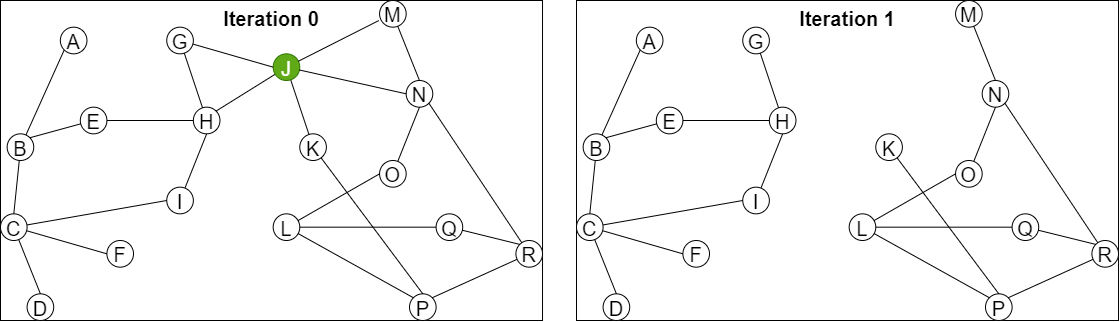
\includegraphics[width=0.9\textwidth]{resilience-process}
		\caption[Network dismantling process]{Network dismantling process. Iteration 1 shows the graph after removing the node with highest degree from original network, thus splitting the graph into two connected components of 9 nodes (left) and 8 nodes (right).}
		\label{fig:resilience-process}
	\end{figure}

This chapter theoretically showed that the influence maximization problem is indeed computationally challenging, which is why this is still an open problem. Next chapter evaluates the same on practical grounds by performing various experiments on a broad range of networks. It is important to note that the proofs presented in this chapter are excerpts from past literature. The notations have been made consistent, the order maintained for completeness, and thorough detail added where needed for reader's convenience.
